\documentclass[aspectratio=169]{beamer}

\usetheme{metropolis}
\usepackage{booktabs}
\usepackage{graphicx}
\usepackage{amsmath}
\usepackage{xcolor}
\usepackage{colortbl}
\usepackage{array}

% Color palette matching the frontier plots
\definecolor{precovid}{RGB}{29,158,117}   % teal  #1D9E75
\definecolor{postcovid}{RGB}{83,74,183}   % purple #534AB7
\definecolor{darkgray}{RGB}{50,50,50}

\setbeamercolor{progress bar}{fg=postcovid}
\setbeamercolor{frametitle}{bg=darkgray}
\setbeamercolor{alerted text}{fg=postcovid}

\title{Efficient Frontier Shift:\\Pre- vs.\ Post-COVID Indian Equities}
\subtitle{IQF Midterm Project}
\author{Viraat Arora \and Yash Khaitan \and Dersh Savla}
\date{2026}

\begin{document}

% ─────────────────────────────────────────────
\maketitle

% ─────────────────────────────────────────────
\begin{frame}{Research Question}
  \begin{block}{}
    \centering\large
    Does the efficient frontier for Indian equities shift meaningfully\\
    between \textbf{pre-COVID (2015--2020)} and \textbf{post-COVID (2021--2024)},\\
    and what structural forces drive the shift?
  \end{block}

  \vspace{1em}
  \textbf{Why it matters}
  \begin{itemize}
    \item COVID was a sharp structural break in global markets
    \item India's equity market saw unprecedented post-pandemic stimulus and sectoral rotation
    \item A shift in the frontier implies a change in the \emph{fundamental} risk-return trade-off available to investors
  \end{itemize}
\end{frame}

% ─────────────────────────────────────────────
\begin{frame}{Dataset}
  \begin{columns}[T]
    \column{0.5\textwidth}
      \textbf{Universe}
      \begin{itemize}
        \item 45 stocks from NIFTY 100 (as of Jan 1, 2015)
        \item Fixed universe $\to$ clean pre/post comparison
        \item Source: Yahoo Finance \texttt{.NS} tickers
      \end{itemize}
      \vspace{0.8em}
      \textbf{Periods (Option C)}
      \begin{itemize}
        \item Pre-COVID: Jan 2015 -- Jan 2020
        \item Crisis window excluded: Feb 2020 -- Jun 2021
        \item Post-COVID: Jul 2021 -- Dec 2024
        \item Analyzed at daily \& weekly frequency
      \end{itemize}

    \column{0.5\textwidth}
      \textbf{Estimation}
      \begin{itemize}
        \item Log returns; annualized ($\times 252$ daily, $\times 52$ weekly)
        \item Ledoit-Wolf shrinkage covariance (accounts for finite-sample noise)
        \item Risk-free rate: RBI 91-day T-Bill yield (pre: 6.54\%, post: 5.78\%)
      \end{itemize}
      \vspace{0.4em}
      \textbf{Data quality}
      \begin{itemize}
        \item Survivorship bias acknowledged: fixed universe biases upward
        \item Delisted/merged tickers retain Yahoo historical data
      \end{itemize}
  \end{columns}
\end{frame}

% ─────────────────────────────────────────────
\begin{frame}{NIFTY 50 Index: 2015--2024}
  \begin{center}
    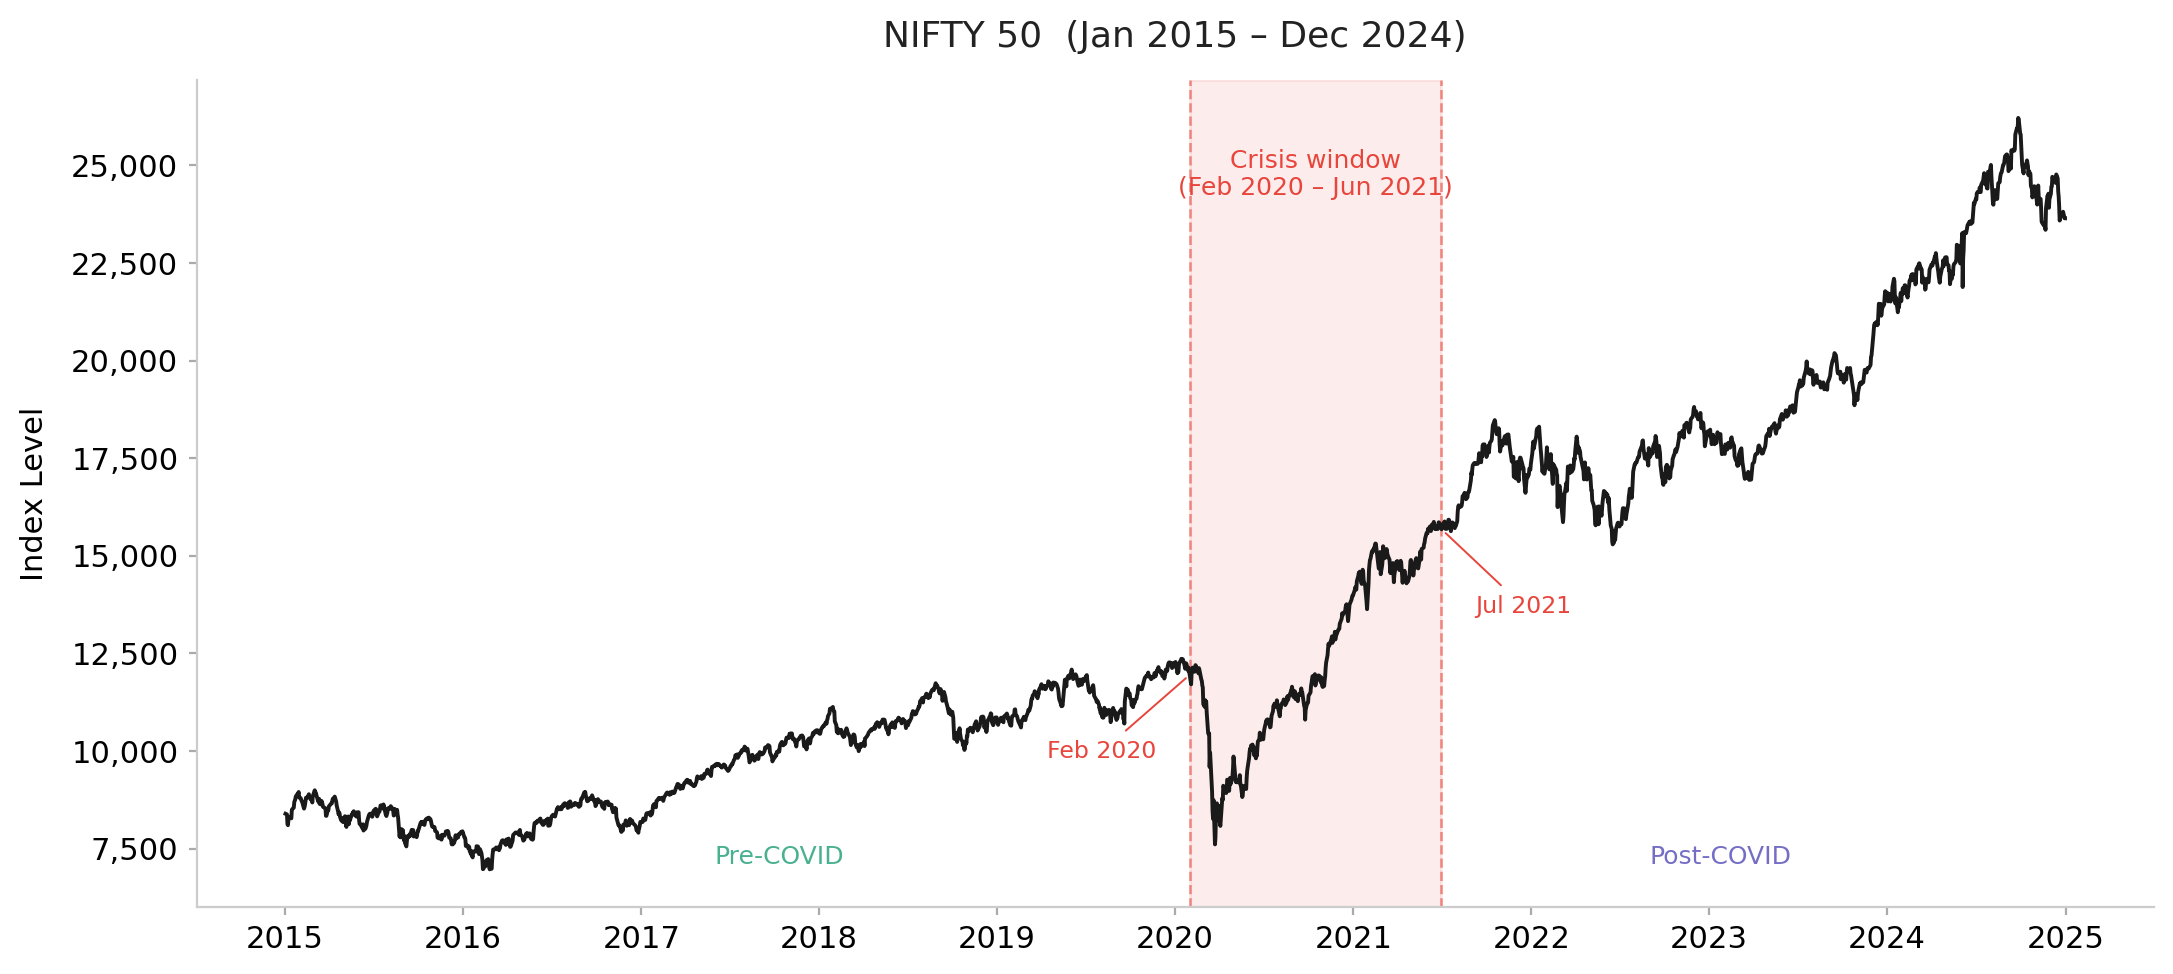
\includegraphics[width=0.90\textwidth]{../Figures/nifty50_timeline.png}
  \end{center}
  \vspace{-0.6em}
  \small
  \begin{itemize}
    \item NIFTY fell $\approx$\,26\% peak-to-trough (Feb--Mar 2020); the crisis window (shaded) is \emph{excluded} from both estimation periods
    \item Post-COVID window captures a clean bull-market regime, free of crash-induced distortions
  \end{itemize}
\end{frame}

% ─────────────────────────────────────────────
\begin{frame}{Methodology}
  \begin{enumerate}
    \item \textbf{Compute statistics} --- log returns annualized; Ledoit-Wolf shrinkage applied to $\boldsymbol{\Sigma}$ for each period
    \vspace{0.4em}
    \item \textbf{Plot individual assets} --- each stock's $(\sigma_i, \mu_i)$ shown as a reference scatter; no simulated feasible set (avoids concentration-of-measure issues at $N=45$)
    \vspace{0.4em}
    \item \textbf{Trace the efficient frontier} --- solve per-point SLSQP optimization
      \[
        \min_{\mathbf{w}}\; \mathbf{w}^\top \boldsymbol{\Sigma}\, \mathbf{w}
        \quad\text{s.t.}\quad \mathbf{w}^\top \boldsymbol{\mu} = \mu^*,\;
        \mathbf{w}^\top \mathbf{1} = 1,\; \mathbf{w} \ge 0
      \]
      sweeping $\mu^*$ from GMV to the highest-return asset
    \vspace{0.4em}
    \item \textbf{Tangency portfolio} --- maximize Sharpe ratio with RBI T-bill as $r_f$; compare pre vs.\ post weights
  \end{enumerate}
\end{frame}

% ─────────────────────────────────────────────
\begin{frame}{Efficient Frontier --- Daily \& Weekly}
  \begin{columns}[T]
    \column{0.5\textwidth}
      \centering
      \textbf{Daily}  \small (T/N $\approx$ 28 pre, 19 post)\\[0.4em]
      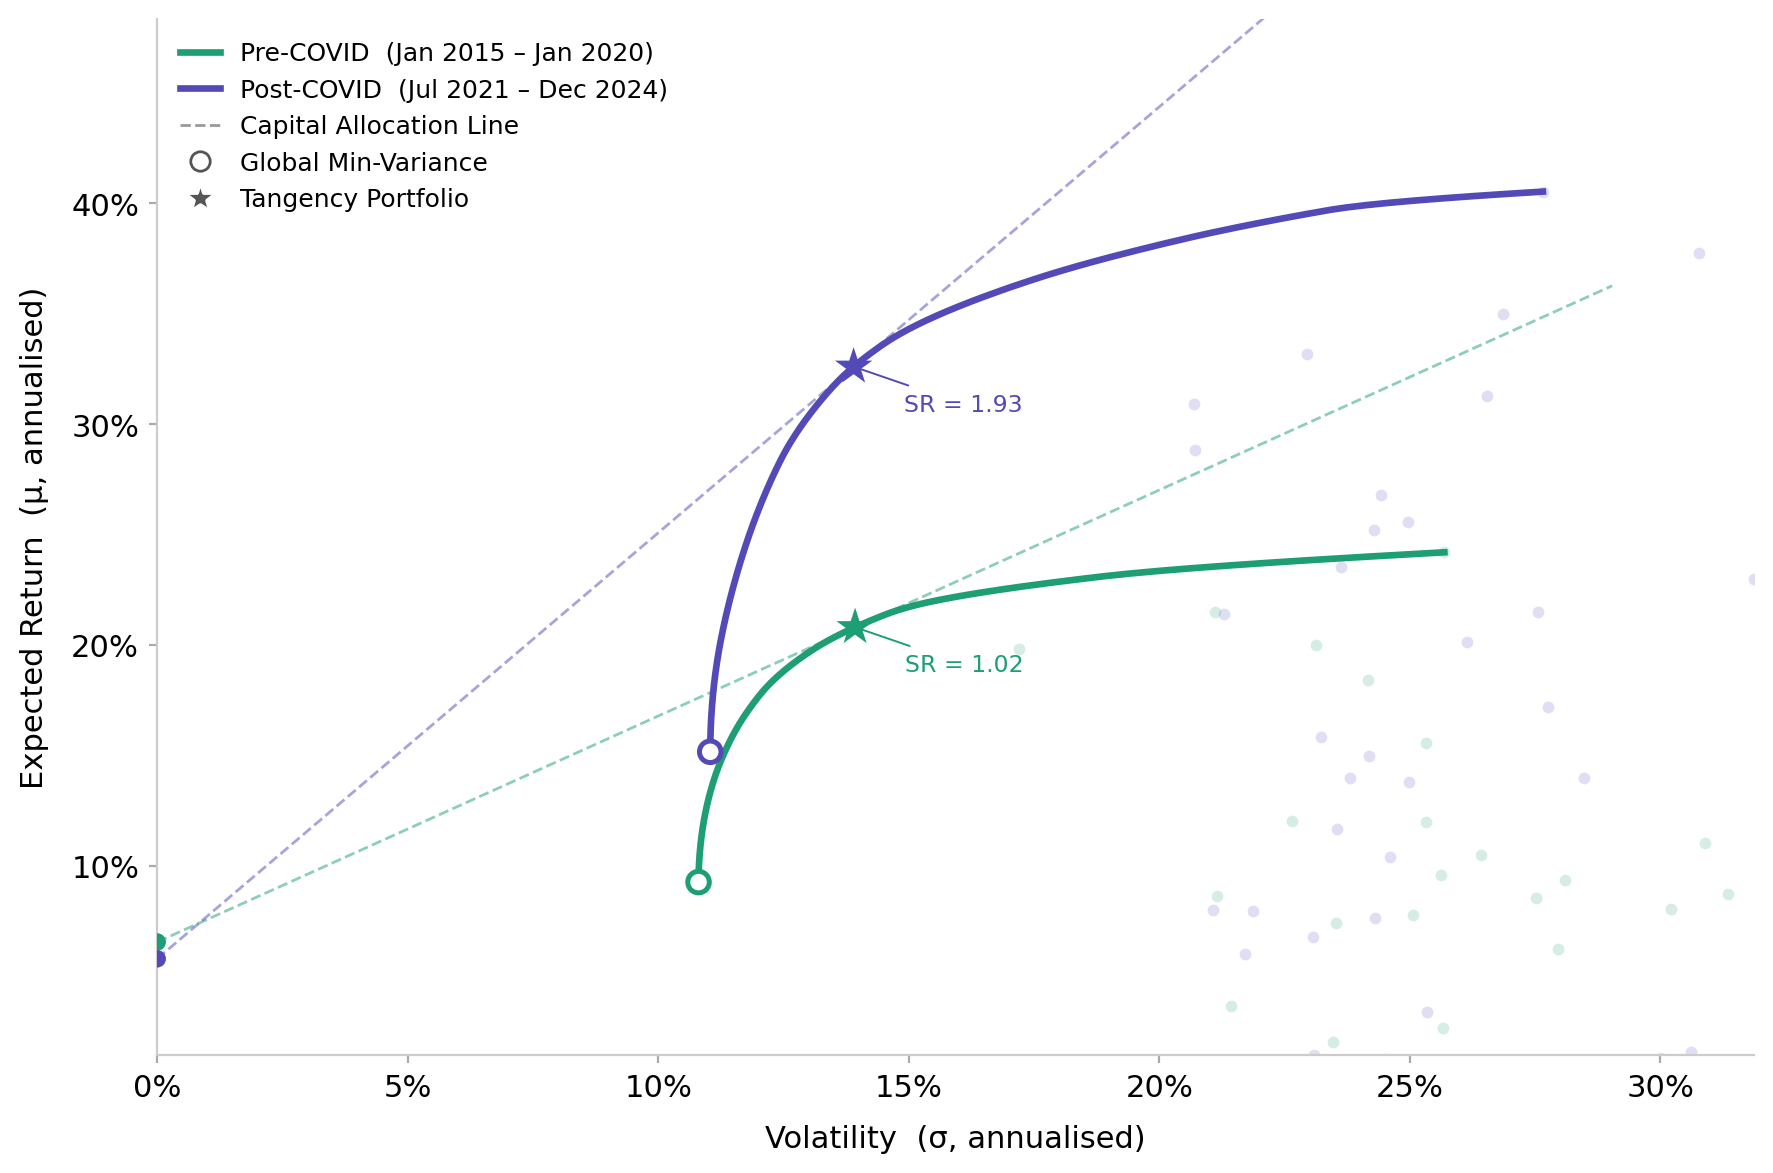
\includegraphics[width=\textwidth]{../Figures/frontier_combined_daily.png}

    \column{0.5\textwidth}
      \centering
      \textbf{Weekly}  \small (T/N $\approx$ 6 pre, 4 post)\\[0.4em]
      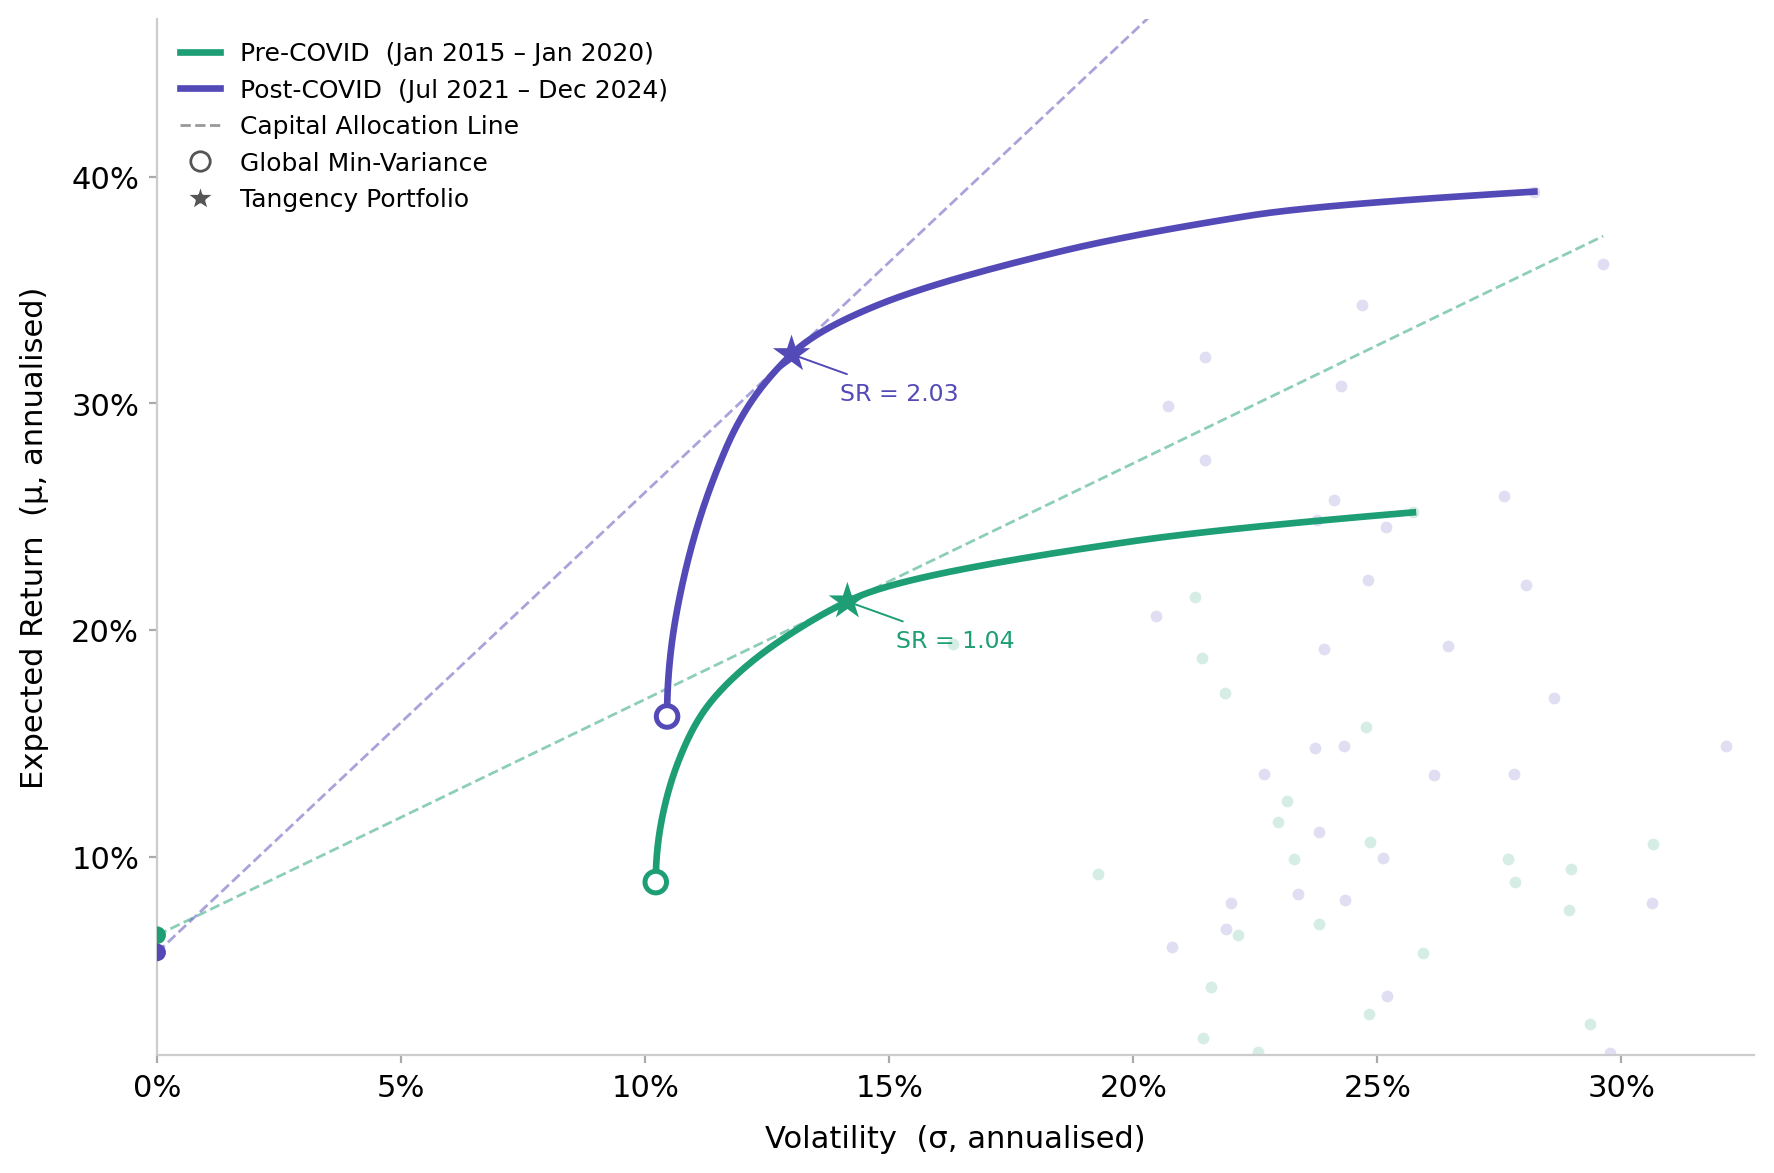
\includegraphics[width=\textwidth]{../Figures/frontier_combined_weekly.png}
  \end{columns}
  \vspace{0.5em}
  \small The post-COVID frontier lies \emph{above and to the right} in both cases --- the risk-return trade-off improved materially.
\end{frame}

% ─────────────────────────────────────────────
\begin{frame}{Tangency Portfolio: Sectoral Rotation}
  \begin{columns}[T]
    \column{0.55\textwidth}
      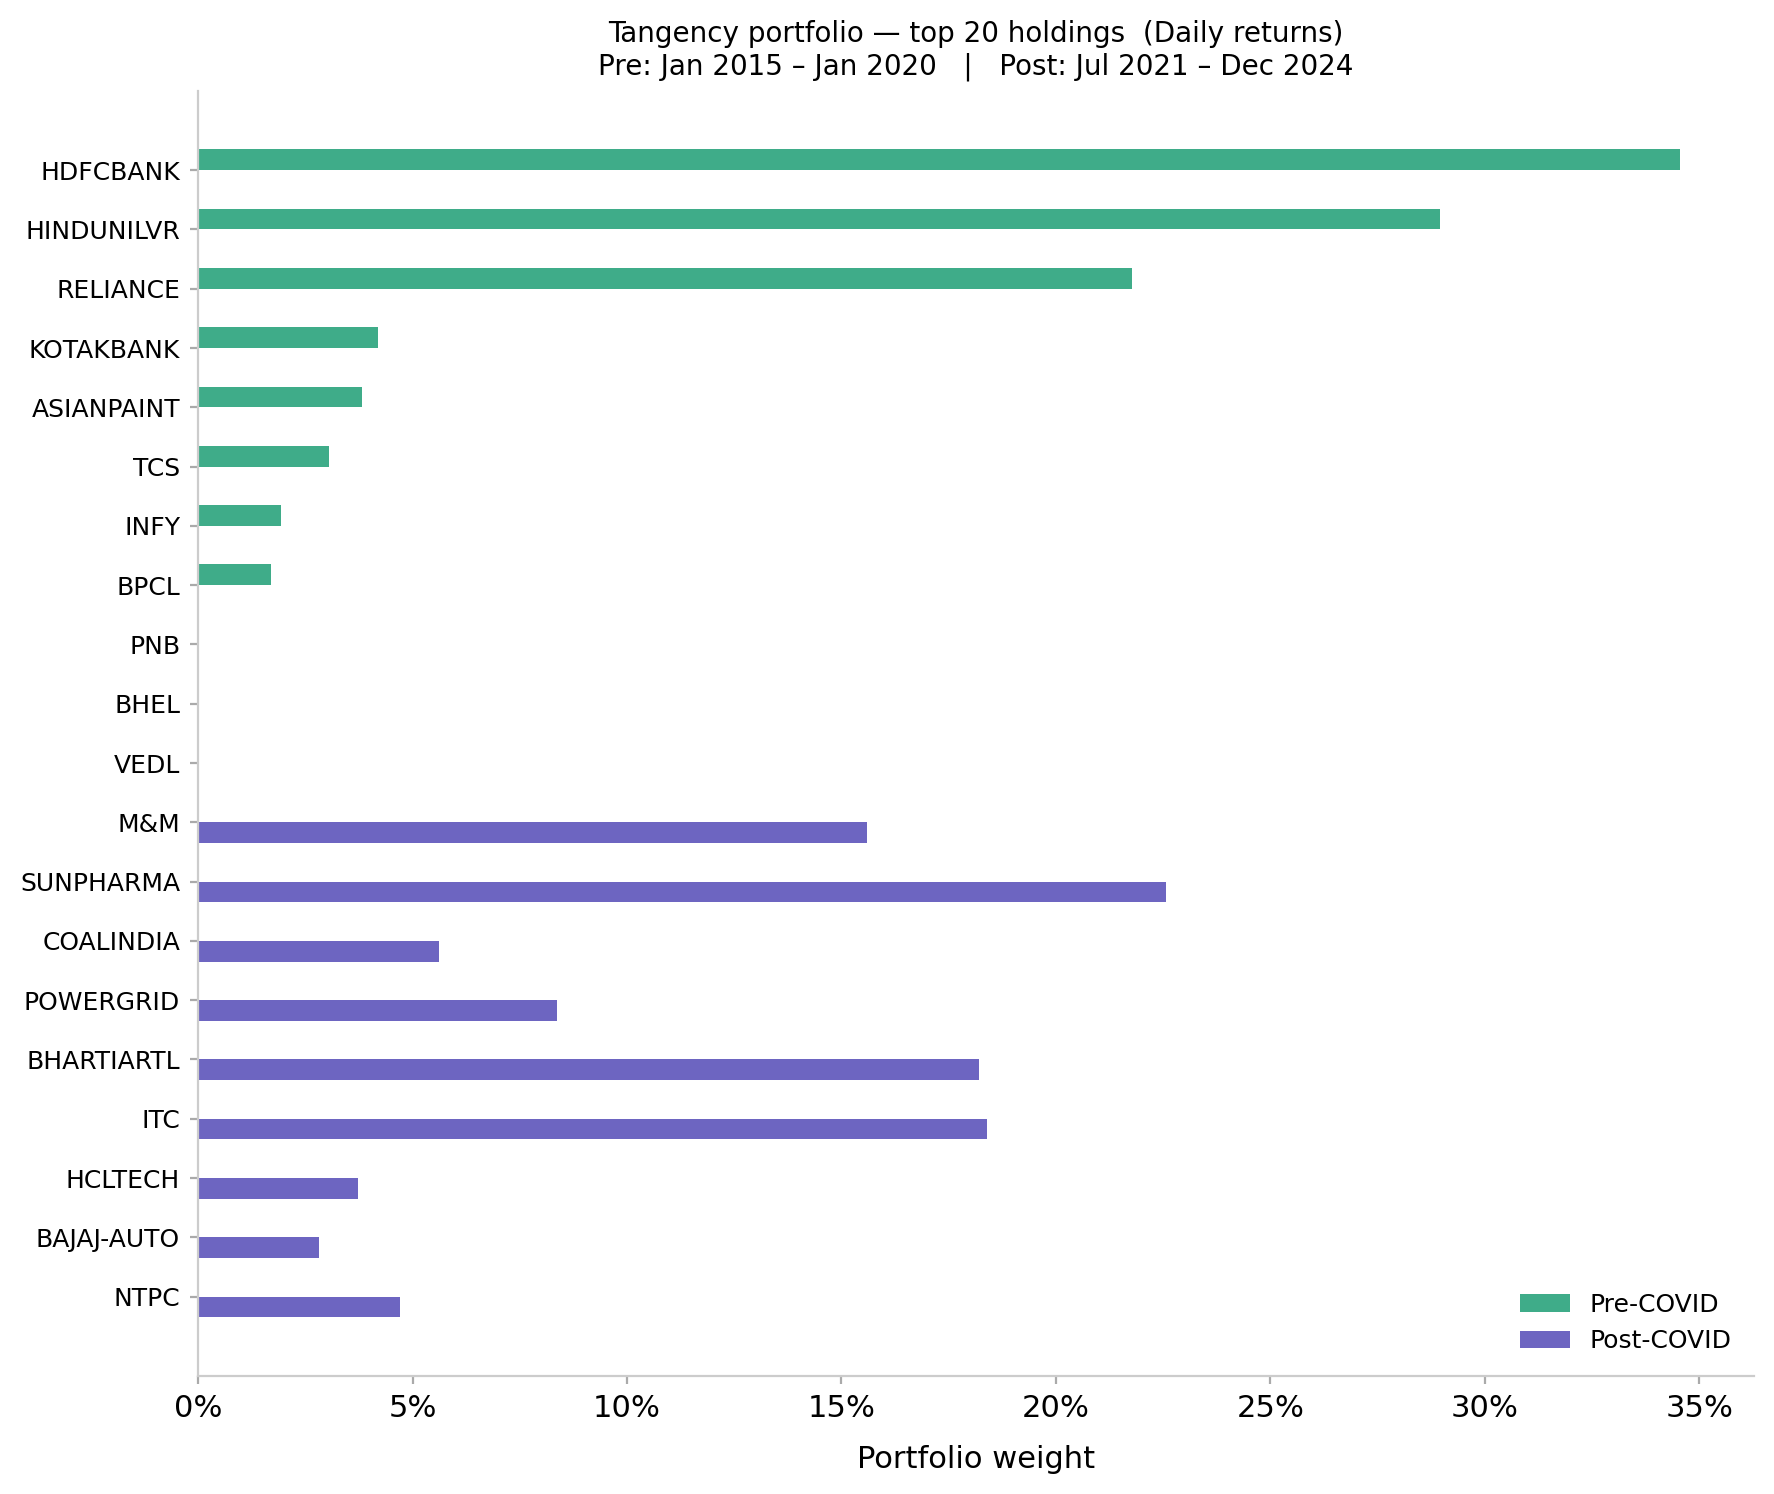
\includegraphics[width=\textwidth]{../Figures/tangency_weights_daily.png}

    \column{0.42\textwidth}
      \small
      \textbf{\textcolor{precovid}{Pre-COVID top holdings}}
      \begin{itemize}\setlength\itemsep{0.1em}
        \item HDFCBANK \hfill 34.5\%
        \item HINDUNILVR \hfill 29.0\%
        \item RELIANCE \hfill 21.8\%
      \end{itemize}

      \vspace{0.6em}
      \textbf{\textcolor{postcovid}{Post-COVID top holdings}}
      \begin{itemize}\setlength\itemsep{0.1em}
        \item SUNPHARMA \hfill 22.6\%
        \item ITC \hfill 18.4\%
        \item BHARTIARTL \hfill 18.2\%
        \item M\&M \hfill 15.6\%
      \end{itemize}

      \vspace{0.7em}
      \small Complete rotation out of \textbf{financials \& FMCG} into \textbf{pharma, telecom, energy, autos} --- the optimizer's view of where the best risk-adjusted returns moved.
  \end{columns}
\end{frame}

% ─────────────────────────────────────────────
\begin{frame}{Interpreting the Shift}
  \textbf{Why did the frontier shift northeastward?}

  \begin{columns}[T]
    \column{0.5\textwidth}
      \textbf{Demand-side drivers}
      \begin{itemize}
        \item Post-COVID fiscal stimulus and infra spending (PLI schemes, BHEL, TATAPOWER)
        \item Domestic retail investor surge: Demat accounts doubled 2020--2022
        \item Foreign capital inflows as India became a China+1 alternative
      \end{itemize}

    \column{0.5\textwidth}
      \textbf{Structural / sectoral drivers}
      \begin{itemize}
        \item Cyclicals and metals outperformed on commodity supercycle (VEDL, HINDALCO, TATASTEEL)
        \item Digital transformation boosted IT returns (HCL, TCS)
        \item Pharma re-rated as strategic post-COVID (SUNPHARMA)
        \item Financials drag: regulatory tightening + HDFC-HDFCBANK merger uncertainty
      \end{itemize}
  \end{columns}
\end{frame}

% ─────────────────────────────────────────────
\begin{frame}{Stock-Level: Biggest Winners}
  \centering
  \begin{tabular}{llrrl}
    \toprule
    \textbf{Ticker} & \textbf{Company} & \textbf{Pre} & \textbf{Post} & \textbf{$\Delta$} \\
    \midrule
    VEDL      & Vedanta                  & $+$8.0\%  & $+$51.2\% & \textcolor{postcovid}{+43.2 pp} \\
    TATAPOWER & Tata Power               & $-$4.9\%  & $+$48.7\% & \textcolor{postcovid}{+53.5 pp} \\
    BHEL      & Bharat Heavy Electricals & $-$20.7\% & $+$46.8\% & \textcolor{postcovid}{+67.5 pp} \\
    M\&M      & Mahindra \& Mahindra     & $+$0.4\%  & $+$43.0\% & \textcolor{postcovid}{+42.6 pp} \\
    SUNPHARMA & Sun Pharmaceutical       & $-$10.4\% & $+$34.1\% & \textcolor{postcovid}{+44.5 pp} \\
    HCLTECH   & HCL Technologies         & $+$8.6\%  & $+$32.4\% & \textcolor{postcovid}{+23.8 pp} \\
    \bottomrule
  \end{tabular}

  \vspace{0.6em}
  \small Industrials, metals, pharma, and IT led the post-COVID recovery.\\
  BHEL and TATAPOWER flipped from worst to top performers --- a full sectoral reversal.
\end{frame}

% ─────────────────────────────────────────────
\begin{frame}{Stock-Level: Pre-COVID Stars That Faded}
  \centering
  \begin{tabular}{llrrr}
    \toprule
    \textbf{Ticker} & \textbf{Company} & \textbf{Pre} & \textbf{Post} & \textbf{$\Delta$} \\
    \midrule
    KOTAKBANK  & Kotak Mahindra Bank & $+$21.1\% & $+$4.6\%  & \textcolor{precovid}{$-$16.5 pp} \\
    HDFCBANK   & HDFC Bank           & $+$19.7\% & $+$10.6\% & \textcolor{precovid}{$-$9.1 pp}  \\
    HINDUNILVR & Hindustan Unilever  & $+$17.9\% & $+$7.9\%  & \textcolor{precovid}{$-$10.0 pp} \\
    ASIANPAINT & Asian Paints        & $+$17.8\% & $+$9.4\%  & \textcolor{precovid}{$-$8.4 pp}  \\
    BPCL       & BPCL                & $+$23.5\% & $+$15.3\% & \textcolor{precovid}{$-$8.2 pp}  \\
    \bottomrule
  \end{tabular}

  \vspace{0.6em}
  \small Financials and consumer staples --- the pre-COVID defensives --- underperformed significantly post-COVID.\\
  These are also the stocks that \emph{dominated the pre-COVID tangency portfolio}.
\end{frame}

% ─────────────────────────────────────────────
\begin{frame}{Robustness Across Frequencies}
  \centering
  \begin{tabular}{lrrrr}
    \toprule
    \textbf{Frequency} & \multicolumn{2}{c}{\textcolor{precovid}{Pre-COVID}} & \multicolumn{2}{c}{\textcolor{postcovid}{Post-COVID}} \\
    \cmidrule(lr){2-3}\cmidrule(lr){4-5}
    & Return & Vol. & Return & Vol. \\
    \midrule
    Daily  \small(T/N $\approx$ 28 / 19)  & 7.91\% & 28.95\% & 24.46\% & 33.17\% \\
    Weekly \small(T/N $\approx$ 6 / 4)    & 7.42\% & 27.95\% & 23.73\% & 32.58\% \\
    \midrule
    \textbf{Avg.\ $\Delta$ Return} & \multicolumn{4}{c}{\textbf{+16.4 pp}} \\
    \textbf{Avg.\ $\Delta$ Vol.}   & \multicolumn{4}{c}{+4.9 pp} \\
    \bottomrule
  \end{tabular}

  \vspace{0.8em}
  The $\approx\!16$ pp return uplift is consistent across both frequencies.\\
  \small Weekly has lower T/N; Ledoit-Wolf shrinkage is higher (0.06--0.07) but the qualitative result holds.
\end{frame}

% ─────────────────────────────────────────────
\begin{frame}{Limitations}
  \begin{itemize}
    \item \textbf{Survivorship bias} --- fixed 2015 universe excludes stocks that failed or were delisted; biases results upward
    \item \textbf{Sample depth} --- daily T/N $\approx$ 19--28 (reliable); weekly T/N $\approx$ 4--6 (higher shrinkage applied, 0.06--0.07); results should be interpreted with this in mind
    \item \textbf{Long-only constraint} --- rules out short selling; actual attainable frontier may be wider
    \item \textbf{Transaction costs \& liquidity} --- not modeled; tangency portfolios are concentrated and may be costly to implement at scale
    \item \textbf{Causal attribution} --- the drivers discussed are correlational; isolating macro causes requires further regression analysis
  \end{itemize}
\end{frame}

% ─────────────────────────────────────────────
\begin{frame}{Future Roadmap}
  \begin{enumerate}
    \item \textbf{Statistical significance test} --- bootstrap or permutation test for the frontier shift; quantify the probability that the observed gap is due to sampling noise
    \vspace{0.4em}
    \item \textbf{Factor attribution} --- decompose the tangency weight rotation into sector and style factors (value, momentum, quality); link the structural shift to identifiable risk premia
    \vspace{0.4em}
    \item \textbf{Transaction cost modeling} --- estimate rebalancing costs for the tangency portfolio; assess whether the Sharpe improvement survives after costs
    \vspace{0.4em}
    \item \textbf{Out-of-sample validation} --- apply post-COVID tangency weights to 2025 data; test whether the frontier shift was a durable regime change or a bull-market artifact
  \end{enumerate}
\end{frame}

% ─────────────────────────────────────────────
\begin{frame}{Conclusions}
  \begin{enumerate}
    \item The efficient frontier for NIFTY 100 equities \textbf{shifted decisively upward and to the right} post-COVID
    \vspace{0.4em}
    \item The return uplift ($\approx$\,+16 pp annualized) \textbf{vastly outpaced the volatility increase} ($\approx$\,+5 pp), improving the risk-adjusted opportunity set
    \vspace{0.4em}
    \item The shift is \textbf{robust across daily and weekly} observation frequencies, with consistent Sharpe improvements
    \vspace{0.4em}
    \item The tangency portfolio underwent a \textbf{complete sectoral rotation} --- financials and FMCG replaced entirely by pharma, telecom, energy, and autos
    \vspace{0.4em}
    \item COVID was not merely a transient shock; it \textbf{structurally altered the investment landscape} for Indian equities
  \end{enumerate}
\end{frame}

% ─────────────────────────────────────────────
\begin{frame}[standout]
  Thank you\\[0.5em]
  \normalsize Questions?
\end{frame}

\end{document}
